%!TEX root = ../main.tex
%%%%%%%%%%%%%%%%%%%%%%%%%%%%%%%%%%
% Links:
%
% Difficulty:
% Companies: 
%%%%%%%%%%%%%%%%%%%%%%%%%%%%%%%%%%


%\begin{figure}
%	\centering
%	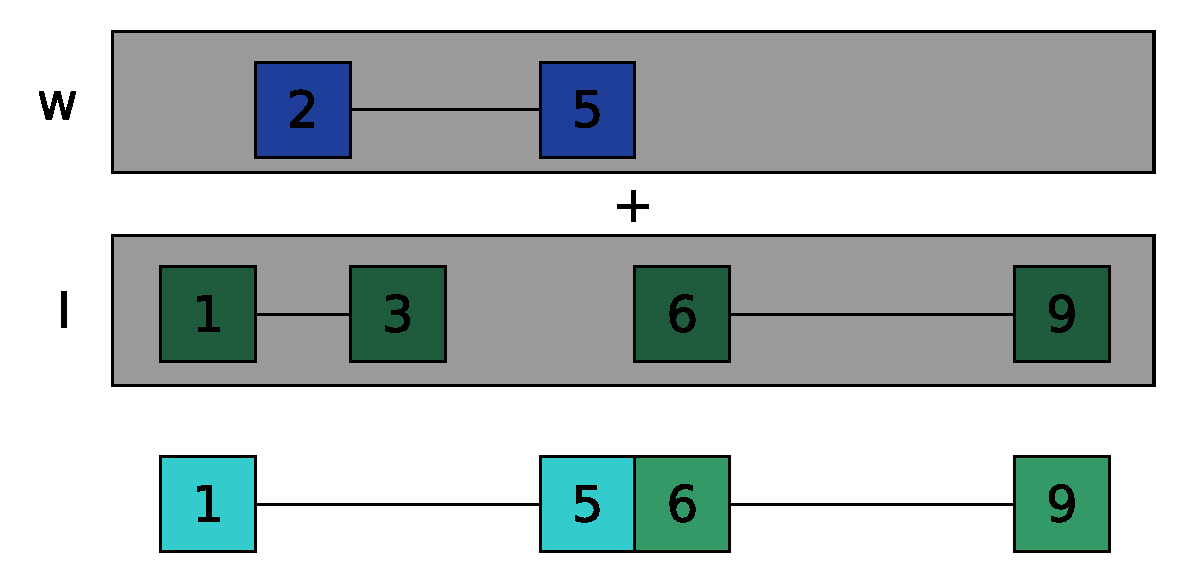
\includegraphics[width=\textwidth]{sources/merge_intervals_2/images/example1}
%	\caption[Sample short cpation]{Sample Caption}.
%	\label{fig:merge_intervals_2:example1}
%\end{figure}

\chapter{Merge Intervals}
\label{ch:merge_intervals_2}
\section*{Introduction}
Intervals are common in programming and they pop-up in numerous applications as they are very versitale and can be used to represent many things, from finite segments in a gemoetry application to time spans for a school timetable.

Intervals are also quite popular in interview questions and this chapter will go through one that is commonly asked at Google where we are asked to, given a list of time intervals, produce a new list where none of the element overlap with another.

We will also investigate a variation of this problem where we are given a list of time intervals where we are guaranteed none of them overlap to begin with and our job is to insert new interval in the list in such a way that the non-overlapping property is maintained. 

\section{Problem statement}
\begin{exercise}
\label{example:merge_intervals_2:exercice1_1}
Write a function that, given a list of intervals $I=\{(s_0, e_0),(s_1, e_1), \ldots,(s_{n-1}, e_{n-1})\}$ represented as a pair of integers, return a copy of the input, $I'$ where all the overlapping intervals have been merged. The resulting list should only contain non-overlapping intervals.

	%example1
	\begin{example}
		\label{example:merge_intervals_2:example1_1}
		\hfill \\
		Given $I=\{(1, 5), (3, 7), (4, 6), (6, 8) \}$ returns $I'=\{(1,8)\}$.
	\end{example}

	\begin{example}
		\label{example:merge_intervals_2:example1_2}
		\hfill \\
		Given $I=\{(1, 5), (6, 7), (4, 4), (9, 12) \}$ returns $I'=\{(1,5),(6,7),(9,12)\}$.
	\end{example}
\end{exercise}

\section{Problem statement}
\begin{exercise}
\label{example:merge_intervals_2:exercice1_2}

Given a sorted list of disjoint (non-overlapping) intervals $I$ and an interval $w$, insert $w$ into $I$ so that the resulting list still contains only disjoint intervals.
You may assume that the intervals are sorted according to their start times.

	%example1
	\begin{example}
		\label{example:merge_intervals_2:example1}
		\hfill \\
		Given $I=\{(1,3),(6,9)\}$ and $w=(2,5)$ the function returns $I'=\{(1,5),(6,9)\}$ (see Figure \ref{example:merge_intervals_2:example1}).
	\end{example}

	%example2
	\begin{example}
		\label{example:merge_intervals_2:example2}
		\hfill \\
		Given $I=\{(1,2),(3,5),(6,7),(8,10),(12,16)\}$ and $w=(4,9)$ the function returns $I'=\{(1,2),(3,10),(12,16)\}$
	\end{example}

\end{exercise}

\begin{figure}
	\centering
	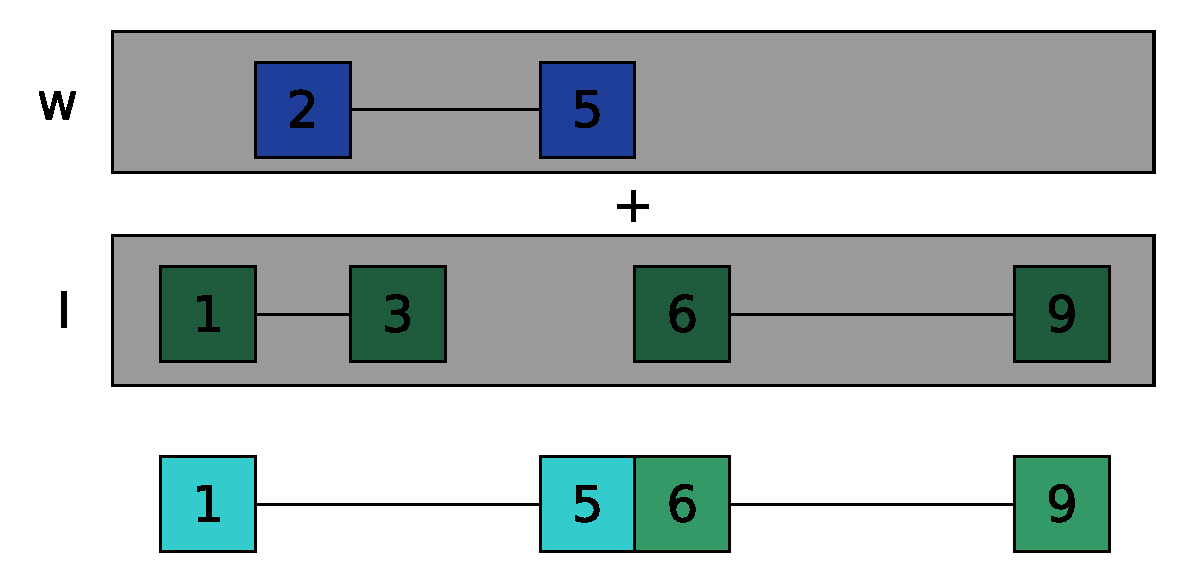
\includegraphics[width=\textwidth]{sources/merge_intervals_2/images/example1}
	\caption[Implicit graph for the Example \ref{example:merge_intervals_2:example1}.]
	{Visual representation the problem instance of Example
	\ref{example:merge_intervals_2:example1}.The \textcolor[HTML]{339966}{$\blacksquare$} green $(1,3)$ and \textcolor[HTML]{3366ff}{$\blacksquare$} blue interval $(2,5)$  are merged together into the \textcolor[HTML]{33cccc}{$\blacksquare$}cyan interval $(1,5)$ below.}
	\label{fig:merge_intervals_2:example1}
\end{figure}



\section{Clarification Questions}

\begin{QandA}
	\item 
	\begin{answered}
		\textit{}
	\end{answered}
	
\end{QandA}

\FloatBarrier

\section{Discussion}
\label{merge_intervals_2:sec:discussion}


\subsection{Brute-force}
\label{merge_intervals_2:sec:bruteforce}

\lstinputlisting[language=c++, caption={Linear time solution.},label=list:merge_intervals_2]{sources/merge_intervals_2/merge_intervals_2_solution1.cpp}

